% !TeX root = ../main.tex
% !TeX encoding = UTF-8
% !TeX spellcheck = none
\subsection{Main Experimental Results}\label{sec:exp-main-results}

This section evaluates RBSRN in terms of overall prediction accuracy, spatial distributions, deviations from routine patterns, and the effects of residual corrections. Comparisons across the full test set and fixed-model diagnostics examine how the two types of correction evidence perform under different traffic conditions.

\subsubsection{Overall Prediction Performance}\label{sec:results-overall}

Tables~\ref{tab:chengdu-inflow}--\ref{tab:shanghai-outflow} compare RBSRN with 13 baseline methods on inflow and outflow forecasting in Chengdu and Shanghai, using positive-target evaluation. Relative changes were calculated from unrounded values against the strongest baseline method for each task and metric. \editorialupdated{Bold and underlined values indicate the best and second-best results in each column, respectively.}

\shanghaiupdated{RBSRN achieved the lowest AVG12 MAE and RMSE on all four tasks. For Chengdu inflow, Chengdu outflow, Shanghai inflow, and Shanghai outflow, AVG12 MAE decreased by 2.00\%, 0.46\%, 1.18\%, and 0.43\% relative to each task's strongest baseline method. AVG12 RMSE decreased by 5.01\%, 1.50\%, 2.33\%, and 0.06\%, respectively, with STGCN, STGCN, HyperD, and HyperD as the corresponding strongest baseline methods.}

Across forecast horizons, RBSRN achieved the lowest MAE and RMSE at H3, H6, and H12 for inflow forecasting in both cities. \shanghaiupdated{For outflow forecasting, HyperD achieved the best H12 MAE in both cities and the best H12 RMSE in Shanghai. RBSRN achieved the lowest errors in all remaining reported comparisons.}

% !TeX root = ../main.tex
% !TeX spellcheck = none
\begin{table}[!htbp]
\centering
\caption{Inflow forecasting results for Chengdu (\(32\times32\) grid)}
\label{tab:chengdu-inflow}
\begingroup
\linespread{1}\fontsize{10}{12}\selectfont
\setlength{\tabcolsep}{4.5pt}
\renewcommand{\arraystretch}{1.05}
\begin{tabular*}{\linewidth}{@{\extracolsep{\fill}}l*{8}{r}@{}}
\toprule
& \multicolumn{2}{c}{H3} & \multicolumn{2}{c}{H6} & \multicolumn{2}{c}{H12} & \multicolumn{2}{c}{AVG12} \\
\cmidrule(l{4.5pt}r{4.5pt}){2-3}\cmidrule(l{4.5pt}r{4.5pt}){4-5}\cmidrule(l{4.5pt}r{4.5pt}){6-7}\cmidrule(l{4.5pt}r{4.5pt}){8-9}
Model & MAE & RMSE & MAE & RMSE & MAE & RMSE & MAE & RMSE \\
\midrule
HA & 1.053 & 1.522 & 1.083 & 1.600 & 1.144 & 1.739 & 1.088 & 1.609 \\
SVR & 0.810 & 1.354 & 0.835 & 1.391 & 0.892 & 1.499 & 0.840 & 1.405 \\
DCRNN (ICLR'18) & 0.725 & \underline{1.321} & 0.790 & 1.363 & 1.025 & 1.574 & 0.829 & 1.399 \\
STGCN (IJCAI'18) & 0.721 & 1.342 & 0.724 & \underline{1.348} & 0.743 & 1.409 & 0.728 & \underline{1.362} \\
GWNet (IJCAI'19) & \underline{0.719} & 1.332 & 0.731 & 1.373 & 0.756 & 1.450 & 0.733 & 1.378 \\
DSTAGNN (ICML'22) & 1.022 & 1.461 & 1.008 & 1.458 & 1.044 & 1.505 & 1.027 & 1.473 \\
PDFormer (AAAI'23) & \pdformerupdated{1.002} & \pdformerupdated{1.443} & \pdformerupdated{1.013} & \pdformerupdated{1.473} & \pdformerupdated{1.030} & \pdformerupdated{1.515} & \pdformerupdated{1.014} & \pdformerupdated{1.473} \\
PatchTST (ICLR'23) & 0.799 & 1.405 & 0.826 & 1.483 & 0.880 & 1.614 & 0.831 & 1.490 \\
TimeMixer (ICLR'24) & 0.818 & 1.434 & 0.844 & 1.505 & 0.895 & 1.620 & 0.848 & 1.510 \\
STDN (AAAI'25) & 1.178 & 1.589 & 1.180 & 1.593 & 1.179 & 1.600 & 1.178 & 1.593 \\
MetaDG (AAAI'26) & 1.102 & 1.564 & 1.170 & 1.678 & 1.291 & 1.882 & 1.178 & 1.692 \\
HyperD (AAAI'26) & 0.723 & 1.369 & \underline{0.723} & 1.369 & \underline{0.726} & \underline{1.382} & \underline{0.723} & 1.369 \\
RAST (AAAI'26) & 0.724 & 1.332 & 0.734 & 1.372 & 0.756 & 1.446 & 0.736 & 1.377 \\
\midrule
\textbf{RBSRN (Ours)} & \textbf{0.704} & \textbf{1.282} & \textbf{0.707} & \textbf{1.290} & \textbf{0.717} & \textbf{1.318} & \textbf{0.708} & \textbf{1.294} \\
\bottomrule
\end{tabular*}
\endgroup
\end{table}

% !TeX root = ../main.tex
% !TeX spellcheck = none
\begin{table}[!htbp]
\centering
\caption{Outflow forecasting results for Chengdu (\(32\times32\) grid)}
\label{tab:chengdu-outflow}
\begingroup
\linespread{1}\fontsize{10}{12}\selectfont
\setlength{\tabcolsep}{4.5pt}
\renewcommand{\arraystretch}{1.05}
\begin{tabular*}{\linewidth}{@{\extracolsep{\fill}}l*{8}{r}@{}}
\toprule
& \multicolumn{2}{c}{H3} & \multicolumn{2}{c}{H6} & \multicolumn{2}{c}{H12} & \multicolumn{2}{c}{AVG12} \\
\cmidrule(l{4.5pt}r{4.5pt}){2-3}\cmidrule(l{4.5pt}r{4.5pt}){4-5}\cmidrule(l{4.5pt}r{4.5pt}){6-7}\cmidrule(l{4.5pt}r{4.5pt}){8-9}
Model & MAE & RMSE & MAE & RMSE & MAE & RMSE & MAE & RMSE \\
\midrule
HA & 1.023 & 1.404 & 1.043 & 1.439 & 1.085 & 1.510 & 1.047 & 1.445 \\
SVR & 0.792 & 1.239 & 0.809 & 1.251 & 0.838 & 1.285 & 0.810 & 1.255 \\
DCRNN (ICLR'18) & 0.714 & \underline{1.230} & 0.761 & \underline{1.237} & 1.151 & 1.642 & 0.844 & 1.326 \\
STGCN (IJCAI'18) & 0.714 & 1.235 & 0.716 & 1.239 & 0.725 & 1.258 & 0.718 & \underline{1.242} \\
GWNet (IJCAI'19) & 0.713 & 1.253 & 0.718 & 1.265 & 0.729 & 1.289 & 0.719 & 1.267 \\
DSTAGNN (ICML'22) & 1.018 & 1.383 & 1.007 & 1.376 & 1.035 & 1.410 & 1.021 & 1.390 \\
PDFormer (AAAI'23) & \pdformerupdated{0.987} & \pdformerupdated{1.365} & \pdformerupdated{0.990} & \pdformerupdated{1.374} & \pdformerupdated{0.997} & \pdformerupdated{1.391} & \pdformerupdated{0.990} & \pdformerupdated{1.374} \\
PatchTST (ICLR'23) & 0.786 & 1.300 & 0.802 & 1.333 & 0.837 & 1.396 & 0.805 & 1.337 \\
TimeMixer (ICLR'24) & 0.807 & 1.315 & 0.823 & 1.345 & 0.856 & 1.404 & 0.826 & 1.349 \\
STDN (AAAI'25) & 1.135 & 1.501 & 1.135 & 1.501 & 1.135 & 1.503 & 1.134 & 1.500 \\
MetaDG (AAAI'26) & 1.082 & 1.471 & 1.139 & 1.543 & 1.245 & 1.672 & 1.146 & 1.550 \\
HyperD (AAAI'26) & \underline{0.712} & 1.249 & \underline{0.712} & 1.249 & \textbf{0.714} & \underline{1.254} & \underline{0.712} & 1.249 \\
RAST (AAAI'26) & 0.718 & 1.242 & 0.724 & 1.257 & 0.735 & 1.282 & 0.724 & 1.258 \\
\midrule
\textbf{RBSRN (Ours)} & \textbf{0.706} & \textbf{1.220} & \textbf{0.708} & \textbf{1.222} & \underline{0.715} & \textbf{1.234} & \textbf{0.709} & \textbf{1.223} \\
\bottomrule
\end{tabular*}
\endgroup
\end{table}

% !TeX root = ../main.tex
% !TeX spellcheck = none
\begin{table}[!htbp]
\centering
\caption{Inflow forecasting results for Shanghai (\(32\times32\) grid)}
\label{tab:shanghai-inflow}
\begingroup
\linespread{1}\fontsize{10}{12}\selectfont
\setlength{\tabcolsep}{4.5pt}
\renewcommand{\arraystretch}{1.05}
\begin{tabular*}{\linewidth}{@{\extracolsep{\fill}}l*{8}{r}@{}}
\toprule
& \multicolumn{2}{c}{H3} & \multicolumn{2}{c}{H6} & \multicolumn{2}{c}{H12} & \multicolumn{2}{c}{AVG12} \\
\cmidrule(l{4.5pt}r{4.5pt}){2-3}\cmidrule(l{4.5pt}r{4.5pt}){4-5}\cmidrule(l{4.5pt}r{4.5pt}){6-7}\cmidrule(l{4.5pt}r{4.5pt}){8-9}
Model & MAE & RMSE & MAE & RMSE & MAE & RMSE & MAE & RMSE \\
\midrule
HA & 1.019 & 1.437 & 1.040 & 1.490 & 1.080 & 1.593 & 1.043 & 1.498 \\
SVR & 0.817 & 1.251 & 0.837 & 1.274 & 0.879 & 1.344 & 0.841 & 1.283 \\
DCRNN (ICLR'18) & \underline{0.734} & \underline{1.243} & 0.748 & 1.262 & 0.808 & 1.328 & 0.758 & 1.272 \\
STGCN (IJCAI'18) & 0.741 & 1.257 & 0.743 & 1.260 & 0.754 & 1.293 & 0.745 & 1.268 \\
GWNet (IJCAI'19) & 0.735 & 1.268 & 0.742 & 1.288 & 0.760 & 1.343 & 0.744 & 1.295 \\
DSTAGNN (ICML'22) & 1.010 & 1.410 & 0.950 & 1.360 & 1.009 & 1.426 & 0.994 & 1.402 \\
PDFormer (AAAI'23) & \pdformerupdated{0.970} & \pdformerupdated{1.356} & \pdformerupdated{0.977} & \pdformerupdated{1.369} & \pdformerupdated{0.995} & \pdformerupdated{1.413} & \pdformerupdated{0.979} & \pdformerupdated{1.376} \\
PatchTST (ICLR'23) & 0.800 & 1.333 & 0.816 & 1.382 & 0.849 & 1.480 & 0.819 & 1.392 \\
TimeMixer (ICLR'24) & 0.821 & 1.331 & 0.836 & 1.372 & 0.868 & 1.463 & 0.839 & 1.381 \\
STDN (AAAI'25) & 1.219 & 1.651 & 1.220 & 1.659 & 1.219 & 1.683 & 1.218 & 1.661 \\
MetaDG (AAAI'26) & 1.082 & 1.517 & 1.168 & 1.624 & 1.421 & 1.944 & 1.201 & 1.667 \\
HyperD (AAAI'26) & 0.737 & 1.261 & \underline{0.737} & 1.261 & \underline{0.737} & \underline{1.263} & \underline{0.737} & \underline{1.260} \\
RAST (AAAI'26) & 0.736 & 1.245 & 0.740 & \underline{1.259} & 0.749 & 1.289 & 0.741 & 1.261 \\
\midrule
\textbf{RBSRN (Ours)} & \shanghaiupdated{\textbf{0.726}} & \shanghaiupdated{\textbf{1.225}} & \shanghaiupdated{\textbf{0.727}} & \shanghaiupdated{\textbf{1.229}} & \shanghaiupdated{\textbf{0.733}} & \shanghaiupdated{\textbf{1.243}} & \shanghaiupdated{\textbf{0.728}} & \shanghaiupdated{\textbf{1.231}} \\
\bottomrule
\end{tabular*}
\endgroup
\end{table}

% !TeX root = ../main.tex
% !TeX spellcheck = none
\begin{table}[!htbp]
\centering
\caption{Outflow forecasting results for Shanghai (\(32\times32\) grid)}
\label{tab:shanghai-outflow}
\begingroup
\linespread{1}\fontsize{10}{12}\selectfont
\setlength{\tabcolsep}{4.5pt}
\renewcommand{\arraystretch}{1.05}
\begin{tabular*}{\linewidth}{@{\extracolsep{\fill}}l*{8}{r}@{}}
\toprule
& \multicolumn{2}{c}{H3} & \multicolumn{2}{c}{H6} & \multicolumn{2}{c}{H12} & \multicolumn{2}{c}{AVG12} \\
\cmidrule(l{4.5pt}r{4.5pt}){2-3}\cmidrule(l{4.5pt}r{4.5pt}){4-5}\cmidrule(l{4.5pt}r{4.5pt}){6-7}\cmidrule(l{4.5pt}r{4.5pt}){8-9}
Model & MAE & RMSE & MAE & RMSE & MAE & RMSE & MAE & RMSE \\
\midrule
HA & 1.059 & 1.528 & 1.079 & 1.559 & 1.118 & 1.629 & 1.082 & 1.565 \\
SVR & 0.866 & 1.373 & 0.882 & 1.395 & 0.914 & 1.447 & 0.883 & 1.398 \\
DCRNN (ICLR'18) & 0.782 & 1.355 & 0.794 & 1.365 & 0.856 & 1.388 & 0.804 & 1.365 \\
STGCN (IJCAI'18) & 0.784 & 1.353 & 0.787 & 1.359 & 0.797 & 1.385 & 0.789 & 1.364 \\
GWNet (IJCAI'19) & 0.783 & 1.381 & 0.788 & 1.394 & 0.801 & 1.424 & 0.789 & 1.396 \\
DSTAGNN (ICML'22) & 1.017 & 1.462 & 0.994 & 1.446 & 1.080 & 1.535 & 1.016 & 1.469 \\
PDFormer (AAAI'23) & \pdformerupdated{1.010} & \pdformerupdated{1.459} & \pdformerupdated{1.017} & \pdformerupdated{1.472} & \pdformerupdated{1.034} & \pdformerupdated{1.511} & \pdformerupdated{1.019} & \pdformerupdated{1.478} \\
PatchTST (ICLR'23) & 0.848 & 1.439 & 0.863 & 1.465 & 0.897 & 1.533 & 0.866 & 1.473 \\
TimeMixer (ICLR'24) & 0.869 & 1.448 & 0.883 & 1.473 & 0.915 & 1.538 & 0.886 & 1.480 \\
STDN (AAAI'25) & 1.109 & 1.591 & 1.107 & 1.593 & 1.105 & 1.605 & 1.106 & 1.595 \\
MetaDG (AAAI'26) & 1.127 & 1.600 & 1.245 & 1.748 & 1.599 & 2.238 & 1.298 & 1.825 \\
HyperD (AAAI'26) & \underline{0.778} & \shanghaiupdated{\underline{1.344}} & \underline{0.778} & \shanghaiupdated{\underline{1.344}} & \textbf{0.778} & \textbf{1.347} & \underline{0.778} & \shanghaiupdated{\underline{1.344}} \\
RAST (AAAI'26) & 0.787 & 1.366 & 0.792 & 1.380 & 0.804 & 1.409 & 0.793 & 1.381 \\
\midrule
\textbf{RBSRN (Ours)} & \shanghaiupdated{\textbf{0.772}} & \shanghaiupdated{\textbf{1.339}} & \shanghaiupdated{\textbf{0.774}} & \shanghaiupdated{\textbf{1.342}} & \shanghaiupdated{\underline{0.779}} & \shanghaiupdated{\underline{1.353}} & \shanghaiupdated{\textbf{0.775}} & \shanghaiupdated{\textbf{1.343}} \\
\bottomrule
\end{tabular*}
\endgroup
\end{table}


The proportion of zero targets is calculated over the same test evaluation positions. For channel \(c\), it is defined as
\begin{equation}
	\rho_c=1-\frac{\sum_{h=1}^{12}|\Omega^{+}_{h,c}|}
	{12N|\mathcal{T}_{\mathrm{test}}|}.
	\label{eq:zero-target-proportion}
\end{equation}
The denominator counts the evaluation positions across all actual test windows, 12 forecast steps, and 1,024 grid cells. When the same timestamp appears in multiple forecast windows, each corresponding forecasting task is counted separately. Table~\ref{tab:metric-scope-sensitivity} reports the zero-target proportions and results under both evaluation scopes for each city and channel.

\textbf{}% !TeX root = ../main.tex
\begin{table}[!htbp]
  \centering
  \caption{Zero-target proportions in the test set and sensitivity of RBSRN to evaluation scope (AVG12)}
  \label{tab:metric-scope-sensitivity}
  \small
  \setlength{\tabcolsep}{5pt}
  \begin{tabular}{llrrrrr}
    \toprule
    City & Channel & Zero targets (\%) & \multicolumn{2}{c}{Positive targets (\(y>0\))} & \multicolumn{2}{c}{\shortstack{All grid cells\\(including zero targets)}} \\
    \cmidrule(lr){4-5}\cmidrule(lr){6-7}
    & & & MAE & RMSE & MAE & RMSE \\
    \midrule
    Chengdu & Inflow & 71.68 & 0.708421 & 1.293545 & 0.936965 & 1.117916 \\
         & Outflow & 70.13 & 0.708654 & 1.223468 & 0.936962 & 1.105671 \\
    Shanghai & Inflow & 64.17 & \shanghaiupdated{0.728085} & \shanghaiupdated{1.230839} & \shanghaiupdated{0.937587} & \shanghaiupdated{1.139290} \\
         & Outflow & 64.94 & \shanghaiupdated{0.774534} & \shanghaiupdated{1.342986} & \shanghaiupdated{0.954306} & \shanghaiupdated{1.184390} \\
    \bottomrule
  \end{tabular}
\end{table}

Table~\ref{tab:metric-scope-sensitivity} compares AVG12 results under positive-target and all-grid evaluation using the same RBSRN checkpoint as the main tables for each city. Zero targets accounted for 64.17\%--71.68\% of evaluation positions across the four tasks. Including these positions increased MAE and decreased RMSE in every task, showing that evaluation scope affects the two metrics differently. Baseline rankings in the main results use positive-target evaluation.

\subsubsection{Spatial Prediction Performance}\label{sec:results-spatial}

\metricrevised{To assess how well RBSRN locates high-flow grid cells, we evaluated predictions 30 minutes after the forecast origin (H6). The analysis covered 1,723 test windows in Chengdu and 1,781 in Shanghai. For each window, we calculated MAE, Spearman rank correlation, and hotspot intersection over union (IoU) over all 1,024 grid cells. Each metric was then averaged over the windows for which it was defined. Inflow and outflow were evaluated separately, and total flow was their cellwise sum. MAE used continuous predictions after inverse standardization, measured in counts per 5 min. Rank correlation assigned average ranks to ties; windows with constant observed flow contributed only to MAE and IoU.}

\metricrevised{Hotspots were defined separately for predicted and observed maps as positive-flow cells within the top \(q\) fraction of the flow ranking. The threshold was the \(\lceil qN\rceil\)-th largest flow value, and all positive values tied at that threshold were included. IoU was the size of the hotspot intersection divided by the size of the union; it was undefined when the union was empty.}

% !TeX root = ../main.tex
\begin{table}[!htbp]
\centering\small
\caption{\editorialupdated{Spatial prediction statistics at H6 across the full test set}}
\label{tab:spatial-fulltest-h6}
\setlength{\tabcolsep}{5pt}
\begin{tabular}{llrrrrrr}
\toprule
City & Flow & Windows & \shortstack{All-grid\\MAE} & Spearman & \shortstack{Valid\\correlations} & IoU$_{10\%}$ & IoU$_{5\%}$ \\
\midrule
Chengdu & Inflow & 1,723 & 0.9366 & 0.4327 & 1,723 & 0.3420 & 0.3495 \\
 & Outflow & 1,723 & 0.9367 & 0.4503 & 1,723 & 0.3356 & 0.3147 \\
 & Total & 1,723 & 1.6750 & 0.5324 & 1,723 & 0.4155 & 0.4142 \\
\midrule
Shanghai & Inflow & 1,781 & \shanghaiupdated{0.9382} & \shanghaiupdated{0.4524} & 1,760 & \shanghaiupdated{0.3224} & \shanghaiupdated{0.3106} \\
 & Outflow & 1,781 & \shanghaiupdated{0.9549} & \shanghaiupdated{0.4920} & 1,759 & \shanghaiupdated{0.3547} & \shanghaiupdated{0.3502} \\
 & Total & 1,781 & \shanghaiupdated{1.6722} & \shanghaiupdated{0.5543} & 1,767 & \shanghaiupdated{0.4068} & \shanghaiupdated{0.4117} \\
\bottomrule
\end{tabular}
\end{table}


\metricrevised{Table~\ref{tab:spatial-fulltest-h6} reports mean spatial rank correlations for total flow of 0.5324 in Chengdu and \shanghaiupdated{0.5543} in Shanghai. At the top 10\% threshold, cells identified as hotspots in both maps accounted for 41.55\% and \shanghaiupdated{40.68\%} of their union on average, respectively. For inflow or outflow evaluated separately, this proportion was \shanghaiupdated{32.24\%--35.47\%}. Tightening the threshold to the top 5\% left the mean total-flow IoU at approximately 0.41 in both cities. Variation between windows at the same horizon was larger. The interquartile ranges of H6 total-flow IoU$_{10\%}$ were 0.270--0.537 in Chengdu and \shanghaiupdated{0.331--0.519} in Shanghai. By comparison, the ranges of mean values over H1--H12 were 0.4122--0.4174 and \shanghaiupdated{0.4048--0.4087}, respectively.}

\metricrevised{Figure~\ref{fig:rbsrn-spatial-h6} shows the spatial distribution of total flow at 08:00 on each city's first complete H6 target day. The Shanghai example had a hotspot IoU of \shanghaiupdated{0.4718}. Its predicted maximum flow was \shanghaiupdated{23.02} counts per 5 min, exceeding the observed maximum of 18 counts per 5 min. In this window, predicted and observed hotspots partially overlapped, but the model overestimated the observed peak flow.}

\begin{figure}[!htbp]
  \centering
  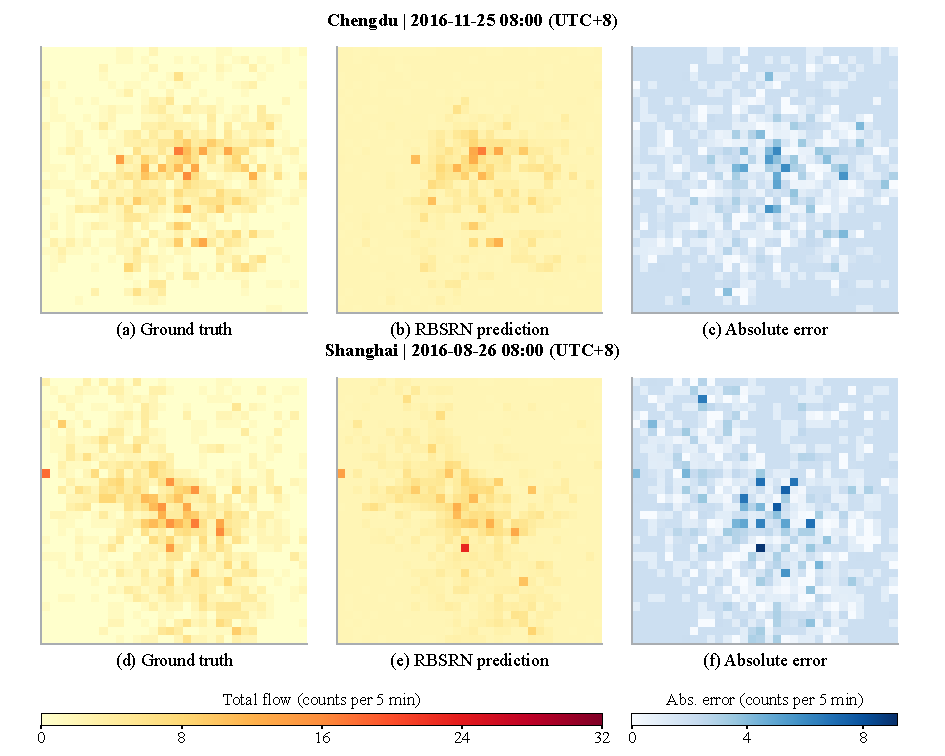
\includegraphics[width=\linewidth]{figures/spatial-fixed-morning.pdf}
  \caption{Example spatial predictions of total flow at H6 (08:00). The top and bottom rows show Chengdu and Shanghai, respectively. The columns show observations, predictions, and absolute errors.}
  \label{fig:rbsrn-spatial-h6}
\end{figure}
\FloatBarrier

% Scenario performance and analyses of the two residual pathways are included in 5.2.
% !TeX root = ../main.tex
% !TeX encoding = UTF-8

\subsubsection{Prediction Performance across Levels of Deviation from Routine Patterns}\label{sec:scenario-performance}\label{sec:exp-scenarios}

All-grid spatial statistics describe flow distribution at a given time. To examine prediction error under deviations from routine levels, we grouped observations by window, grid cell, and channel. At positions with positive H6 target flow, RBSRN was compared with 16 baselines. Chengdu scenario analysis and the subsequent residual diagnostics use a dedicated diagnostic checkpoint, whose full-test-set H6 MAE is 0.709952 for inflow and 0.709944 for outflow. The main Chengdu tables use the comparison checkpoint. Shanghai scenario analysis and residual diagnostics use the epoch-115 checkpoint reported in the main tables.

The routine-flow reference is the median training flow for the same grid cell, channel, 5-minute slot, and weekday/weekend type. We used deduplicated training-history timestamps that passed the quality checks. If a slot had fewer than four observations for one day type, the two types were pooled; if it had none, we used the grid-cell and channel median. We divided each observation's difference from its reference by a robust scale to obtain the standardized residual \(r_k\). The scale is the training residual median absolute deviation multiplied by 1.4826, with a lower bound of 1 count. The input-window deviation score is \(D=\frac{1}{12}\sum_{k=1}^{12}|r_k|\). For each city and channel, we pooled grid cells from training windows whose 12 historical steps passed the quality checks. The 50th, 80th, and 95th percentiles of \(D\) define four groups (Table~\ref{tab:scenario-group-thresholds}); boundary values enter the lower group.

% !TeX root = ../main.tex
\begin{table}[!htbp]
  \centering\footnotesize
  \caption{Scenario-group thresholds from training data}
  \label{tab:scenario-group-thresholds}
  \setlength{\tabcolsep}{4pt}
  \begin{tabular}{llrrrrrr}
    \toprule
    City & Channel & \(D_{50}\) & \(D_{80}\) & \(D_{95}\) & \(U_{75}\) & \(B_{1/3}\) & \(B_{2/3}\) \\
    \midrule
    Chengdu & Inflow & 0.166667 & 0.583333 & 1.083333 & 1.636364 & 0.279326 & 0.453125 \\
    Chengdu & Outflow & 0.166667 & 0.625000 & 1.083333 & 1.636364 & 0.287192 & 0.471179 \\
    Shanghai & Inflow & 0.281038 & 0.708333 & 1.096048 & 1.636364 & 0.311065 & 0.489387 \\
    Shanghai & Outflow & 0.250000 & 0.674491 & 1.083333 & 1.590909 & 0.311294 & 0.492517 \\
    \bottomrule
  \end{tabular}
\end{table}


\begin{figure}[!htbp]
  \centering
  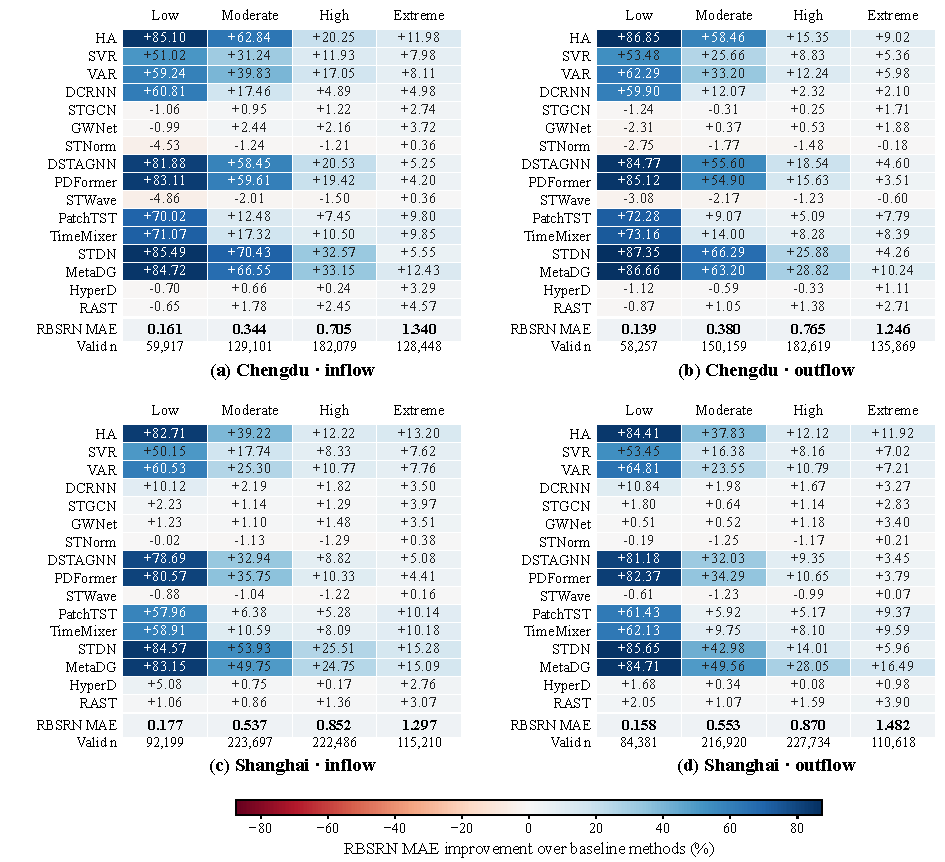
\includegraphics[width=\linewidth]{figures/scenarios/performance_h6_paper.pdf}
  \caption{RBSRN relative MAE at H6 across deviation groups.}
  \label{fig:scenario-performance}
\end{figure}

Figure~\ref{fig:scenario-performance} compares methods within each group; positive values indicate an MAE reduction relative to the corresponding baseline. In the Extreme group, RBSRN had the lowest MAE for Chengdu inflow, Shanghai inflow, and Shanghai outflow, with reductions of 0.36\%, 0.16\%, and 0.07\% relative to STWave. For Chengdu outflow, RBSRN ranked third, with MAE 0.60\% above STWave. STWave and STNorm had lower errors than RBSRN in the Moderate and High groups on all four tasks.

Absolute MAE increased with deviation level on all four tasks. Extreme-group MAE was 7.33--9.37 times the Low-group value. For Chengdu inflow, MAE increased from 0.161 to 1.340 while mean positive-target flow increased from 1.160 to 3.637 counts per 5 min, so the group differences reflect both deviation level and flow magnitude.

\subsubsection{Effects of SERR Residual Corrections across Recent-Change Scenarios}\label{sec:scenario-serr}

Within the high-deviation subset combining High and Extreme observations (\(D>D_{80}\)), recent-change intensity is defined by successive differences in historical standardized residuals:
\begin{equation}
  U=\frac{1}{11}\sum_{k=2}^{12}|r_k-r_{k-1}|.
  \label{eq:scenario-recent-change}
\end{equation}
The 75th percentile of \(U\) among high-deviation training samples separates Slow and Rapid groups; values above the threshold enter Rapid.

We examined each residual correction with a fixed-model residual-removal diagnostic. Model parameters, gates, and all other outputs were held fixed while one specified correction was subtracted from the final prediction:
\begin{equation}
  \Delta\mathrm{MAE}_{e}
  =\mathrm{MAE}(\widehat Y-C_e)-\mathrm{MAE}(\widehat Y),
  \label{eq:scenario-residual-removal}
\end{equation}
Here, \(C_e\) is the signed correction added to the prediction, including the original gating weight, learnable strength coefficient, and inverse-standardization scale. Removing the SERR self-evolution expert subtracts its weighted difference from the base prediction; removing the directed time-lagged expert subtracts its weighted correction; removing BCMS subtracts the full cross-region correction. Gating weights retain their original values and are not renormalized. A positive difference means that the correction reduced group-average MAE. Because the loss is nonlinear, differences for separate corrections are not additive. This diagnostic complements the independently retrained ablations in Section~\ref{sec:exp-ablation}: it measures sensitivity of one fixed model, whereas the ablations compare retrained configurations.

In Figure~\ref{fig:scenario-serr}, all 16 removal differences across the eight city--channel--change groups were positive. The self-evolution correction benefit in Rapid was 1.15--2.82 times the Slow-group benefit, whereas the directed time-lagged correction was smaller. Its Rapid-group benefit was higher than its Slow-group benefit in Chengdu and lower in Shanghai.

\begin{figure}[!htbp]
  \centering
  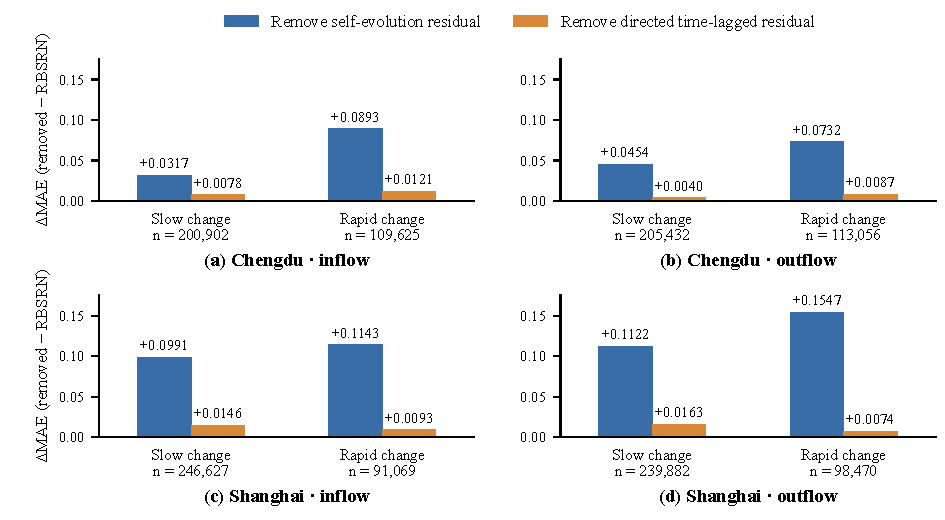
\includegraphics[width=0.92\linewidth]{figures/scenarios/serr_sensitivity_h6_paper.pdf}
\caption{H6 SERR residual-removal sensitivity by recent-change group.}
  \label{fig:scenario-serr}
\end{figure}

\subsubsection{Effects of BCMS Residual Corrections across Background Discrepancies and Forecast Horizons}\label{sec:scenario-bcms}

We measured source--target background similarity with a history-derived discrepancy proxy. Let \(\mathcal C_i\) denote the valid fixed candidate-source set for target cell \(i\), and let \(\bar r_i\) be its mean standardized residual over the 12 historical steps. For each channel, define
\begin{equation}
  B_i=\frac{1}{|\mathcal C_i|}\sum_{j\in\mathcal C_i}|\bar r_i-\bar r_j|.
  \label{eq:scenario-background-difference}
\end{equation}
The candidate set follows the model's fixed support. \(B_i\) describes discrepancy in the observed history and is separate from the low-frequency representation learned by BCMS. Tertile thresholds estimated from high-deviation training samples define Low, Medium, and High discrepancy groups (Table~\ref{tab:scenario-group-thresholds}). We removed the full BCMS correction at H1--H12 using Eq.~\eqref{eq:scenario-residual-removal}. Both figures report MAE changes in \(10^{-3}\) counts per 5 min; each cell is \(1000\times\Delta\mathrm{MAE}\).

Figure~\ref{fig:scenario-bcms} shows a consistent ordering across city, channel, and horizon: the mean benefit was largest in the Low group, followed by Medium and High. Of 144 background-group--horizon cells, 143 were positive; the only negative value was approximately \(-4.8\times10^{-6}\) for Chengdu outflow in the High group at H5. Benefits varied across horizons without a monotonic trend.

\begin{figure}[!htbp]
  \centering
  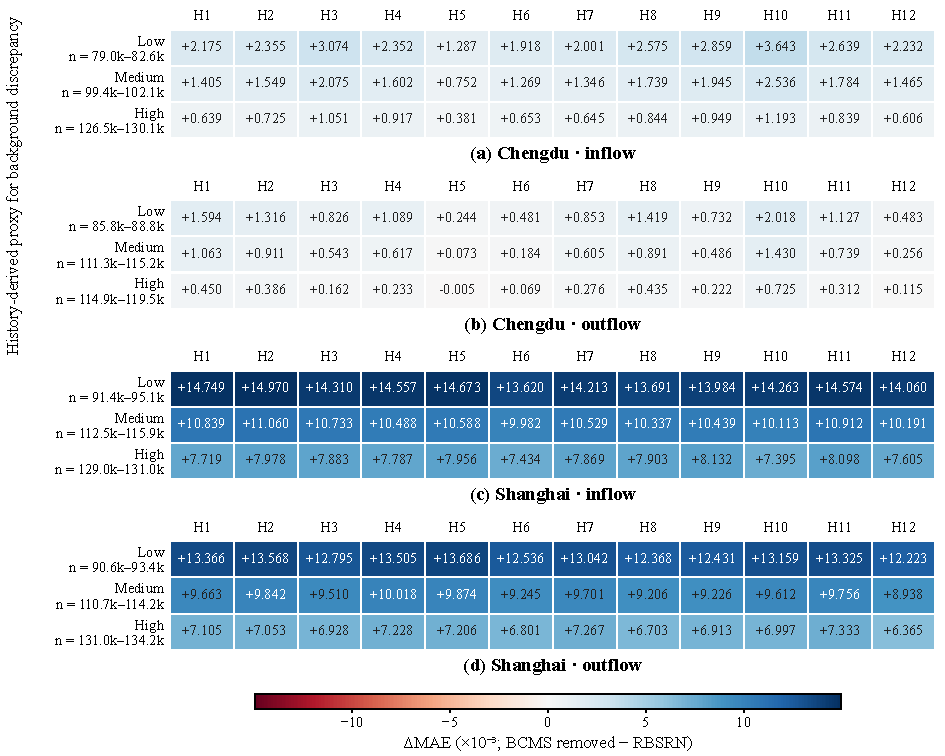
\includegraphics[width=0.92\linewidth]{figures/scenarios/bcms_sensitivity_horizons_paper.pdf}
\caption{BCMS residual-removal sensitivity in high-deviation scenarios.}
  \label{fig:scenario-bcms}
\end{figure}

Figure~\ref{fig:scenario-bcms-all} extends the analysis to the full test set with the same thresholds fitted from high-deviation training histories. All 144 removal differences were positive and exceeded the corresponding high-deviation values. The Low--Medium--High ordering persisted. For Shanghai inflow at H6, full-test differences were 0.025547, 0.015634, and 0.009873, compared with 0.013620, 0.009982, and 0.007434 in the high-deviation subset. The full-test analysis therefore shows that the average BCMS benefit extends beyond high-deviation samples.

\begin{figure}[!htbp]
  \centering
  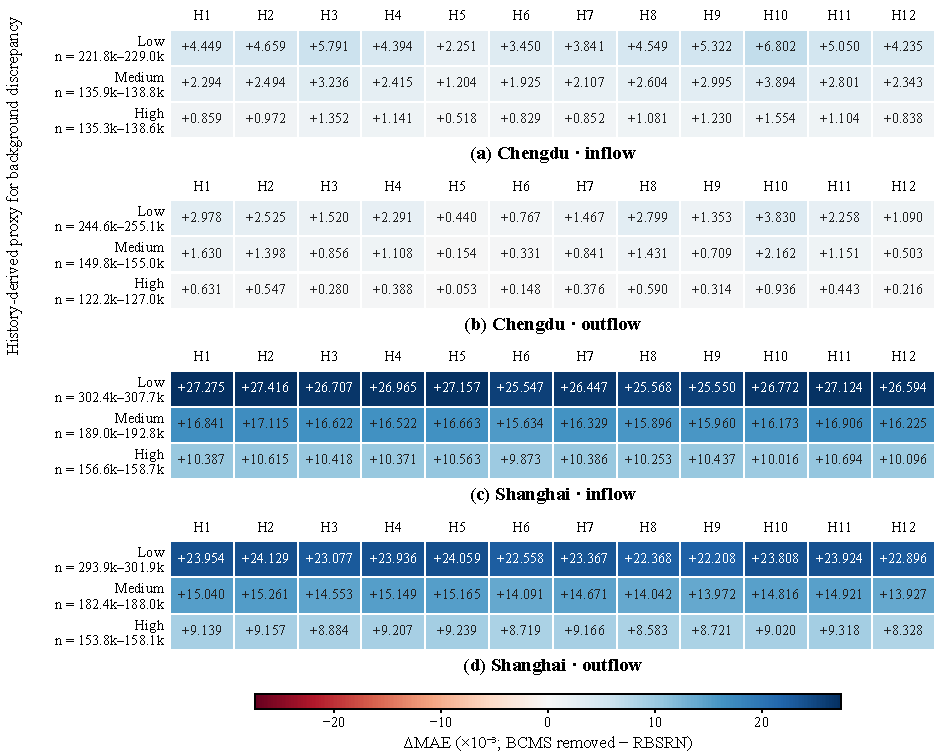
\includegraphics[width=0.92\linewidth]{figures/scenarios/bcms_sensitivity_horizons_all_test_paper.pdf}
\caption{BCMS residual-removal sensitivity across the full test set.}
  \label{fig:scenario-bcms-all}
\end{figure}

